\documentclass[conference,compsoc]{IEEEtran}
% Some/most Computer Society conferences require the compsoc mode option,
% but others may want the standard conference format.
%
% If IEEEtran.cls has not been installed into the LaTeX system files,
% manually specify the path to it like:
% \documentclass[conference,compsoc]{../sty/IEEEtran}





% Some very useful LaTeX packages include:
% (uncomment the ones you want to load)


\ifCLASSOPTIONcompsoc
  % IEEE Computer Society needs nocompress option
  % requires cite.sty v4.0 or later (November 2003)
  \usepackage[nocompress]{cite}
\else
  % normal IEEE
  \usepackage{cite}
\fi


\usepackage{listings}
\usepackage{amsmath,amssymb,amsfonts}
\usepackage{algorithm}
\usepackage{algpseudocode}
\usepackage{graphicx}
\usepackage{textcomp}
\usepackage{xcolor}
\usepackage{listings}
\usepackage{tikz}
\usetikzlibrary{positioning, arrows.meta}
\usepackage{url}
\usepackage{xcolor}
\usepackage{soul}
\usepackage{lstcoq}
\def\BibTeX{{\rm B\kern-.05em{\sc i\kern-.025em b}\kern-.08em
    T\kern-.1667em\lower.7ex\hbox{E}\kern-.125emX}}
\begin{document}
\title{Hope}

\author{Anonymous}

% make the title area
\maketitle

% As a general rule, do not put math, special symbols or citations
% in the abstract
\begin{abstract}
  \st{Despite the recent growth of zero-knowledge succinct argument 
  of knowledge (ZkSNARK)}, 
  $\Sigma$-protocol remains a popular choice in electronic voting to maintain privacy 
  and verifiability of elections and still used in prominent e-voting systems such as 
  Helios, Belenois, SwissPost, etc. However, 
  the existing implementations of sigma protocol have two 
  shortcomings: (i) the same code is written twice, once for the front-end (JavaScript/TypeScript)
  and once for the back-end (Python/OCaml/Java), which is time-consuming but more importantly error-prone, 
  and (ii) none of these implementations offer any security guarantees. 
  
  In this paper, we present a certified implementation of sigma protocol in the Coq theorem prover and
  prove our implementation is (special) sound, complete, and 
  (special honest-verifier) zero-knowledge. Moreover, 
  we compile our Coq formalisation to WebAssembly and Rust; 
  thereby solve the problem of writing the same code twice. 
  We demonstrate the applicability of our
  formalisation by encoding the sigma protcol implemented in 
  Helios, Belenois, and SwissPost voting systems. 
  \st{Our long terms goal is to provide a verified cryptographic library that can be 
  readily used in privacy-preserving voting systems.}
\end{abstract}

% no keywords




% For peer review papers, you can put extra information on the cover
% page as needed:
% \ifCLASSOPTIONpeerreview
% \begin{center} \bfseries EDICS Category: 3-BBND \end{center}
% \fi
%
% For peerreview papers, this IEEEtran command inserts a page break and
% creates the second title. It will be ignored for other modes.
\IEEEpeerreviewmaketitle



\iffalse
\section{How to pitch this paper and What is the unique selling point of our work?}
Our Coq formalisation can be used at front-end (WebAssembly code) and 
back-end (Rust). Contrary to the existing work, our formalisation
does not write the same code twice. But sigma protocol is arcane and has 
been formalised couple of times before so why another formalisation?
None of the formalisation has been able to extract the code to executable code 
and one that was able to do so did not reason about probabilities in an intuitive way.
Moreover, that work was just geared towards verifying a transcript rather than
constructing it. Also, recently ZKP community started a movement to 
formalise the sigma protocols. We also demonstrates the 
applicability of our formalisation by encoding Helios cryptographic protocols
in our formalisation. 



\textbf{We need to explain why formal verification is important in the context of voting systems.}

\begin{itemize}
  \item Explain zero-knowledge proofs (completeness, soundness, zero-knowledge)
  \item Explain sigma protocols (completeness, special-soundness, honest-verifier zero-knowledg) 
  and mention about the Schnorr protocol
  \item Our contribution
  \item Explain the Schnorr protocol
  \item Explain Parallel, And, Eq, Or, and NEQ relations (also explain that 
  most of the formalisation has worked on And and Or relations)
\end{itemize}

\fi






\section{Introduction}
Electronic voting offers convenience and efficiency in electoral processes, potentially improving 
accessibility for disabled voters, increasing participation among overseas voters, and lowering 
the costs associated with conducting elections. Moreover,
they can streamline the voting process, reduce administrative burdens, and enable 
faster tallying of results. However, electronic voting also brings significant 
challenges in ensuring the privacy and verifiability, a must for free-and-fair elections, of the voting process. Therefore, 
privacy and verifiability are two crucial elements that a voting system must ensure.
In a paper-ballot election, privacy is maintained by 
ensuring that no identifying information is present on a ballot that links it to a particular voter, 
and verifiability is achieved through scrutineers closely observing various electoral processes, 
including the counting of ballots. In order to have a similar effect in electronic voting, encryption 
is employed to safeguard the privacy of voter choices, while publicly verifiable evidence 
(such as zero-knowledge proofs) allows voters and independent observers to verify the integrity of 
the voting process. However, no matter how advanced the cryptographic techniques, they are useless 
if their software implementation contains bugs. In fact, 
the Swiss Federal Chancellery suspended electronic voting in 2019 because of 
a fatal software bug in the implementation of a cryptographic primitive 
that allowed someone to change the cast votes without being detected \cite{9152765}!
It only resumed in 2023 after getting feedbacks from academic 
community \cite{swiss_evoting_chronik} about the various components used in 
the electronic voting software. However, it is not an isolated  
instance where bugs have been found in a voting software, e.g., 
Voatz \cite{255334} (used in West Virginia, USA election),
Democracy Live Online Voting System \cite{263858} 
(used in Delaware, West Virginia, and New Jersey, USA election), 
Moscow Internet Voting System \cite{10.1007/978-3-030-51280-4_3}
(used in Russia election), and iVote System \cite{10.1007/978-3-319-22270-7_3, 10.1145/3014812.3014837} 
(used in New South Wales, Australia election), etc. 
These unfortunate situations can largely be attributed to two factors: 
(i) closed source code (proprietary artifacts) because most of these bugs were 
discovered by researchers who inspected the code after they were made public, and 
(ii) software testing which is inadequate to rule out all the bugs 
from a software. Therefore, to avoid the situations like this, 
an electronic voting system must adhere to \textit{software independence}\cite{rivest2008notion}:
\begin{quote}
  A voting system is software-independent if an
  (undetected) change or error in its software cannot
  cause an undetectable change or error in an
  election outcome. 
\end{quote}
\noindent
Therefore, many electronic voting systems follow the principals 
of \textit{end-to-end verifiability}. End-to-end verifiability is 
defined as: 
\begin{itemize}
  \item \textit{cast-as-intended}: voters get proof that the electronic ballot accurately reflects their choices.
  \item \textit{collected-as-cast}: the election authority provides proof that the electronic ballots are received without tampering.
  \item \textit{counted-as-collected}: the election authority provides proof that the results are based on correctly counting all received ballots.
\end{itemize} 


Finally, voters and scrutineers inspect these proofs and accept or reject the election results based on 
the verification of these proofs. In practice, this means that during the execution of an election, 
electronic voting software generates data, and voters and scrutineers verify the conformity of 
this data using independently written computer programs. The rationale is that if there is 
any discrepancy in the electronic voting system, at least one scrutineer or voter would detect it.
It is important to note that end-to-end verifiability is a valuable feature because it 
allows for the verification of the election results by checking the proofs of correctness 
once the election has concluded. This ensures that the election process was conducted 
properly and that the results are accurate, but it is only in action during or after the voting has taken place.
However, can we use it as a guiding principle to develop an electronic voting software, way before 
an election? The answer is yes; we can use a formal language to express end-to-end verifiability, or parts of 
it, and develop various components of an electronic voting 
software in this formal language. This process is called formal verification, or correct-by-construction,
and it ensures that the software always produces valid proofs that 
are accepted by voters and scrutineers every time. In other words, formal verification
can be employed to develop reliable electronic voting software.
In fact, formal verification has emerged as a promising solution 
to eliminate potential bugs from software, and in recent years it has been increasingly 
adopted in real-world software applications \cite{10.1145/1111037.1111042}, 
including cryptography \cite{8835346,10.1145/3133956.3134043,190894,10.1145/2701415,
10.1145/2660267.2660370,10.1145/3319535.3363211}.

In this paper, we present a certified implementation of $\Sigma$-protocol --an efficient 
type of zero-knowledge proof-- and its Parallel, And, Eq, Or, and Neq compositions in 
the formal language of the Coq proof assistant. 
We have formalised and analysed the interactive version of 
$\Sigma$-protocol, but in practice it is not convenient due to the required interaction. 
Therefore, all $\Sigma$-protocol implementations use the \textit{Fiat-Shamir} 
transformation \cite{10.5555/36664.36676} to make them non-interactive. 
Fiat-Shamir transformation replaces the randomness of the public-coin verifier by 
a cryptographic hash function, though 
some care is required \cite{10.1007/978-3-642-34961-4_38}.
Therefore, we have encoded SHA-256 in Coq, with the usual correctness properties \cite{nist_fips_180_4},
to make our formalisation self-contained and independent of external libraries. Additionally, we 
have implemented efficient arithmetic procedures for prime field and the Schnorr group to 
ensure our library is usable. \textcolor{blue}{Finally, we extract WebAssembly and 
Rust code from our certified implementation, one of the novelties of our 
formalisation}.


There are numerous implementations of  $\Sigma$-protocol in various languages, 
e.g., Helios is written in Python \cite{helios_crypto}, Belenois is written in OCaml \cite{belenios_core}, 
and SwissPost is written in Java \cite{swisspost_crypto_primitives}.
However, there are two main issues with these implementations: 
(i) the same code is written twice 
once for the front-end (JavaScript, TypeScript) and once for the back-end (Python, OCaml, or Java) and 
 (ii) more importantly, none of these implementations offer any formal guarantees about the code.
Unlike Helios and SwissPost,
we write one implementation and extract WebAssembly (front-end) and Rust (back-end) (\textcolor{red}{Todo: using the MetaCoq library}).
Belenois is slightly different in this respect and uses $Js\_of\_ocaml$ \cite{js_of_ocaml}
to compile the OCaml code into JavaScript so it has only one 
implementation written in OCaml; nonetheless it is not verified 
and offers no formal guarantees. To the best of our knowledge, 
this is the first formal verification of sigma protocol that can be used at 
the front-end (WebAssembly code) and back-end (Rust code). 

\subsection{Outline}
Outline goes here. 


\section{Sigma Protocol}\label{sigma_protocol}
Despite the recent growth and popularity of zero-knowledge succinct 
argument of knowledge (ZKSNARK), $\Sigma$-protocol remains a
leading cryptographic proof system in privacy-preserving voting systems. 
$\Sigma$-protocol is used in Helios --a widely popular voting system-- \cite{adida2008helios}, 
Belenois --used in French elections for overseas 
voters\footnote{VVFE, used in French elections, is a derivative of (part of) Belenios and 
inherited all the zero-knowledge proofs from Belenois.}-- \cite{cortier2023french}, and 
SwissPost --used in Swiss elections for overseas voters-- voting 
systems \cite{10.1007/978-3-031-15911-4_4} (\textcolor{red}{Look for more examples}). 
Moreover, recently zero-knowledge proof community started a movement to standardise
the sigma protocol \cite{ZKProof}.
One of the main reasons for its popularity in privacy-preserving voting systems is its
well-understood security.  Other application of sigma protocol 
include identification schemes, (\textcolor{red}{cite more work}). 

%\textbf{Introduce here that sigma protocol is efficient and simple and all other details about sigma protocol.} 
Zero-knowledge proofs were first studied by Goldwasser, Micali, and Rackoff \cite{10.1145/22145.22178} and 
are possible for all problems in $NP$ \cite{10.1145/116825.116852}. Recall that $NP$ is the class of 
problems that have efficient verifiers; that is, for a given problem in the $NP$ class, there is 
a polynomial-time algorithm that can verify whether a given solution, or witness, to the problem is correct or not.
More formally, for a given $NP$-relation $R$ and a statement $x$, zero-knowledge proof allows a prover 
$P$ to convince a verifier $V$ that they posses a witness $w$ --polynomial in length of $x$-- such 
that ($x$, $w$) $\in$ $R$. To achieve this, $P$ and $V$ engage in a 
interactive protocol and  at the end of the protocol $V$ either accepts or rejects the proofs.
\textit{Sigma protocol}, shown in the figure \ref{fig:sig_picture}, is an efficient three move zero-knowledge proof where the 
verifier is assumed to be honest and characterised by completeness, (special) soundness, and 
(special honest-verifier) zero-knowledge. More formally: 
\begin{itemize}
  \item \textbf{Completeness:}
  when $P$ and $V$ follow the protocol, $V$ always accepts. 
  In other words, if $P$ knows $w$ for $x$ such that ($x$, $w$) $\in$ $R$,  
  then $P$ can successfully construct a proof $(a, c, r)$ that always passes the verification equation, 
  i.e., $V$ accepts. 

\item \textbf{Special soundness:}
there exists a polynomial-time extractor $E$ which given 
two accepting transcripts $(a, c, r)$ and $(a, c', r')$ for $x$, 
it can extract a witness $w$ such that $(x, w) \in R$. In other words, 
if $P$ does not know $w$ for $x$ then it cannot construct a proof 
(a; c; r) that will passes the verification check. 
\item \textbf{Special honest-verifier zero-knowledge proof:}
There exists a polynomial-time simulator $S$ that, for any 
$v \in L_R$ where $L_R = \{x  \mid (x, w) \in R\}$,
generates an accepting transcript $(a, c, r)$ 
without using the witness $w$. 
This transcript is indistinguishable from one produced by an 
honest conversation between $P$ and $V$ using $w$, 
satisfying $(v,w) \in R$.

\end{itemize}


\begin{figure}[ht]
  \centering
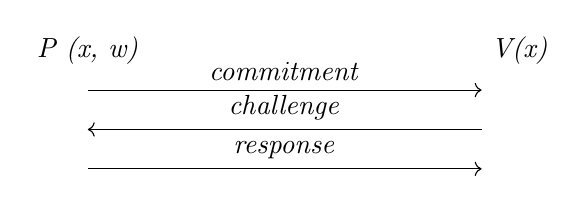
\begin{tikzpicture}
  \node (Prover)  {\textit{P (x, w)}} (0,0);
  \node (Verifier) [right=of Prover] at (4, 0) {\textit{V(x)}};
  % First arrow (left to right)
  \draw[->] (0,-0.5) -- (5,-0.5) node[midway, above] {\textit{commitment}};
  
  % Second arrow (right to left)
  \draw[->] (5,-1) -- (0,-1) node[midway, above] {\textit{challenge}};
  
  % Third arrow (left to right)
  \draw[->] (0,-1.5) -- (5,-1.5) node[midway, above] {\textit{response}};
\end{tikzpicture}
\caption{Sigma Protocol}
\label{fig:sig_picture}
\end{figure}







Sigma protocol was first defined by Ronald Cramer \cite{cramer1996modular} 
and the first efficient sigma protocol was introduced by Schnorr in \cite{schnorr1991efficient}. 
Eventhough there exists many sigma protocols, the Schnorr protocol is used extensively in privacy-preserving voting systems, e.g, Helios, Belenois, SwissPost, etc. Therefore, 
our formalisation is geared towards the Schnorr protocol. 
Moreover, we also formalise the composition of (i) $n$ \textit{Parallel} Schnorr, 
(i) $n$ \textit{And} Schnorr, (iii) $n$ \textit{Or} Schnorr, and (iv) $n$ \textit{Eq} Schnorr protocol. 
Ideally, given the abstraction of our formlisation (\textit{vector space}), we could have 
abstracted the sigma protocol and their composition in a generic way \cite{10.1007/978-3-642-02384-2_17},
but we decided to focus on the Schnorr protocol and its composition to ensure familiar APIs 
for e-voting in WebAssembly and Rust. We also formalise Okamoto protocol as a subprotocol 
for Neq composition (\textbf{Berry: does it sound okay?}). However, we have not seen 
much use of Neq in the privacy-preserving voting systems, at least in the existing voting systems. 




\section{The Coq Theorem Prover}
\textcolor{red}{FIXME:this seems too much of tutorial Coq so let me know your thoughts. We 
can explain MetaCoq here as well and the extraction to Rust and WebAssembly
so that it justifies this tutorial}
The Coq theorem prover \cite{the_coq_development_team} is a computer program that interacts with users, 
enabling them to encode mathematical definitions, express specifications (true statements) about 
their definitions, and formally prove that the definitions imply the specifications. 
A user first defines their mathematical object (definition) and then figure 
out some  true statements (specifications) about 
that object. Once the user has definition 
and specifications, they need to prove 
that the definition satisfies the specifications 
(proof writing). In general, amongst these three steps, 
the proof writing step is the most challenging and important step. 
During the proof writing, an user interacts with the Coq theorem prover 
via \emph{tactics}, a domain specific language 
to ease the proof writing. Even though the Coq theorem 
provides some amount of automation and proof 
search, most of the time it requires human assistance to finish the proof. 
It is one the most popular and robust theorem, and
one of reasons for its popularity is 
dependent types, that makes it possible to encode
any mathematical statement in its logic.
It has been used to verify many real world software projects and mathematical 
artefacts. For example, Coq has been used to 
formally verify CompCert \cite{10.1145/1111037.1111042}, 
a C compiler used by many companies\footnote{https://www.absint.com/partners.htm}, 
Fiat-Crypto \cite{8835346} 
used in BoringSSL --a cryptographic library used in Chrome, Android, 
and CloudFlare--, ConCert \cite{10.1145/3372885.3373829}, 
a smart contract certification framework, etc. \textbf{FIXME: More examples}



\subsubsection*{Definitions, Specifications, and Proofs}
In this section, we demonstrate how to encode definitions, write specifications,
and formally prove that definitions satisfy the specifications 
in the Coq theorem prover by an example of 
natural numbers (natural numbers is the set $\{0, 1, 2, 3, \dots \}$). 
The set of natural numbers $Nat$ is the set of elements defined by the 
following clauses:
\begin{itemize}
  \item \emph{Zero}, represents $0$, is in the set Nat ($Zero \in Nat$)
  \item if $n$ is in the set Nat, then \emph{Succ n}, represents $n + 1$, 
    is also in the set Nat (if $n \in Nat$, then $Succ \text{ }n \in Nat$)
\end{itemize}

\noindent 
This representation of natural numbers is called 
inductively defined set where the base case, or starting point,
is Zero (constant symbol), and if we have a natural number $n$, then we can 
get the next natural number by prefixing Succ (unary function symbol) to $n$.  
Using this encoding of natural numbers, we can represent 
$1$ by \emph{Succ Zero}, and $2$ by \emph{Succ (Succ Zero)}, 
and so on. We encode the set \emph{Nat} in Coq as inductively defined data type, 
shown in Listing \ref{ind_nat}, with 
two constructors: \emph{Zero} and \emph{Succ}. 
\begin{lstlisting}[frame=single, language=Coq, caption={Definition of Natural Number},
  label={ind_nat},captionpos=t, basicstyle=\ttfamily\footnotesize,
  abovecaptionskip=-\medskipamount]
Inductive Nat : Type := 
| Zero : Nat 
| Succ : Nat -> Nat.
\end{lstlisting}


With the definition of natural numbers at our disposal,
we can define addition, subtraction, multiplication, division, and 
many other mathematical functions on natural numbers in the Coq theorem prover. 
However, we only define the addition function,
shown in Listing \ref{add_fn}, to demonstrate the concept. 
In Coq, \emph{Fixpoint} is a keyword 
for defining function, followed by the name of the function (\emph{plus}), 
arguments (\emph{m} and \emph{n}), and the body (definition) of the function.
The body of plus shown in Listing \ref{add_fn} is Coq encoding of the 
following two clauses: 
\begin{enumerate}
  \item plus Zero n = n 
  \item plus (Succ m) n = Succ (plus m n)
\end{enumerate}  

\noindent 
The first clause amounts to $0 + n = n$ and the second clause
amounts to $ (1 + m) + n = 1 + (m + n)$.


\begin{lstlisting}[frame=single, language=Coq, caption={Addition of two Natural Numbers},
  label={add_fn},captionpos=t, basicstyle=\ttfamily\footnotesize,
  abovecaptionskip=-\medskipamount]
Fixpoint plus (m n : Nat) :=
  match m with
  | Zero => n
  | Succ m' => Succ (plus m' n)
  end.

\end{lstlisting}

So far, we have defined natural numbers and addition. Now, we will specify 
some properties of addition on natural numbers. Mathematically, addition 
is known to be associative and commutative. For simplicity, we will 
prove that our addition definition is commutative, as shown in 
Listing \ref{plus_comm}, which serves as the specification for our 
addition operation.

\begin{lstlisting}[frame=single, language=Coq, caption={Addition is Commutative},
  label={plus_comm},captionpos=t, basicstyle=\ttfamily\footnotesize,
  abovecaptionskip=-\medskipamount]
Theorem plus_commutative : 
  forall n m, plus n m = plus m n. 
Proof.
  induction n.
  (* base case *)
  + intros m.
  (* proof terms omitted *)
  (* inductive case *)  
  + intros m.
    rewrite IHn.
    (* proof terms omitted *)
Qed.
  
\end{lstlisting}

In Coq, \emph{Theorem} is the keyword used to define a specification, 
followed by the name (\emph{plus\_comm}). This specifies that for any 
two natural numbers $m$ and $n$ (encoded as \texttt{forall n m}), 
adding $n$ to $m$ is the same as adding $m$ to $n$ 
(encoded as \texttt{plus n m = plus m n}).
To write a formal proof of this statement, we start by indicating that 
we will use the tactic language with the keyword \emph{Proof}. Once the 
proof is complete, we use the keyword \emph{Qed} to signal to Coq that 
our proof is finished. At this point, Coq verifies that the proof is complete 
and correct according to its logic. If the proof is not finished, Coq will 
not accept \emph{Qed}. Therefore, having a \emph{Qed} for any specification 
ensures that our proof is correct, provided we trust the Coq theorem prover.
However, at this point, the curious reader can argue that why should we trust 
Coq because it is a computer program, similar any other computer program? 
Trust in Coq relies on two factors: (i) its meta-theory, the 
\emph{Calculus of Inductive Constructions} \cite{thierry1988calculus}, and 
(ii) its implementation in OCaml \cite{the_coq_development_team}.
The meta theory of Coq has been scrutinised for decades
by many mathematicians and so far it has withstood all 
the scrutiny, but not so much for its OCaml implementation \cite{coq_critical_bugs}. 
Therefore, there is a recent effort to develop more 
rigorous implementation for Coq proof checking \cite{10.1145/3371076} \textbf{FIXME: this is the place 
to state that we are following this path of MetaCoq and extraction}.


\subsection{Web Assembly and Rust from the Coq Formalisation (MetaCoq)}
  Bas






\subsection{Schnorr Protocol Coq Encoding}
  We briefly explain the Schnorr protocol, an interactive protocol 
  between a prover and a verifier, which follows the same structure as 
  depicted in Figure \ref{fig:sig_picture}. 
  Given some public input $G = (g, q, h)$ where $G$
  is a cyclic group of prime order $q$, $g$ and $h$ are two 
  generators of the group $G$, the prover claims that they know a
  witness $w$ for the statement $h = g^w$; the existence of such
  a $w$ is immediate because $g$ generates the group. However,
  does the prover know the witness $w$? In order to convince the
  verifier, the prover and the verifier do the following:
  \begin{itemize}
    \item the prover picks a random number $u$, computes $a = g^u$,
    and sends $a$ to the verifier.
    \item the verifier picks a random challenge $c$ and sends it to
    the prover
    \item the prover computes $r = u + c * w$ and sends $r$ to the
    verifier
  \end{itemize}

The verifier accepts the transcript $(a, c, r)$ if $g^r = a * h^c$, otherwise rejects. We can prove that 
this protocol has completeness, special soundness, and special honest-verifier 
zero-knowledge proof. 


\begin{itemize}
  \item completeness: when $P$ and $V$ both follows the protocol, $V$ accepts the proof, i.e., 
  the verification equation checks out. We can see by algebraic simplification that it is the case.
    \begin{align*}
      g^r = g^{u + c * w} = g^u * (g^w)^c = a * h^c
    \end{align*}
  \item special soundness: from two accepting 
  conversations $(a, c, r)$ and $(a, c', r')$ where $c \neq c'$,
  a polynomial-time extractor can extract a witness $w$, 
  which is equal to $(r - r') * (c - c')^{-1}$, 
  such that $g^w = h$. By means of algebraic simplification, 
  we can see that it is the case.  
  \begin{align}
    g^r = a * h^c = g^u * (g^w)^c = g^{u + w * c}  \\
    g^{r'} = a * h^{c'} = g^u * (g^w)^{c'} = g^{u + w * c'}
  \end{align}
  Diving the expression (1) with (2), we get
  \begin{align*}
    g^{(r-r')} = g^{w * (c - c')}
  \end{align*}
  and multiplying both sides by $(c - c')^{-1}$ we 
  get 
  \begin{align*}
    g^{(r-r') * (c - c')^{-1}} = g^{w}
  \end{align*}

  \item special honest-verifier zero-knowledge proof:
   the distribution for the conversations with an honest verifier --involving witness $w$--
   and the conversation with a simulator --without witness $w$-- are the same, given a 
   challenge $c$. We can 
   see this algebraically that both distributions \ref{f} and \ref{snd} have the identical 
   distribution, i.e., $1/q$. 
   \begin{align}\label{f}
    \{(a, c, r) \mid u \in_{R} Z_q ; a := g^u; r := u + c * w \}
   \end{align}
   \begin{align}\label{snd}
    \{(a, c, r) \mid u \in_{R} Z_q ; a := g^r * h^{-c}\}
   \end{align}
   
\end{itemize}


In the Schnorr protocol, the elements $g$, $h$, and $a$ are group elements from the underlying group, while $u$, $c$, and $r$
are scalar values from the underlying prime field. In practice, both the group elements and the field elements are large 
numbers modulo some prime numbers, although the operations on them differ. 
One possibility is to encode the Coq functions to work with concrete numbers from the underlying group and field, 
but this leads to cumbersome proofs because of dealing with concrete numbers, but the bigger problem 
is that it is not modular. For most programming languages, this distinction 
may not be significant, but it can be a potential source of bugs \cite{10.1007/978-3-662-63958-0_24}. 
However, when encoding it in Coq, we need to thoroughly detail these distinctions because 
the same large number can belong to a group or field and that dictates what operations are available for them. 
Therefore, to avoid this unpleasant situation,  
we decided to abstract the underlying group as an abstract type $G$, endowed with 
usual group operation, and the underlying field as an abstract type $F$, endowed with 
filed operation in our formalisation. Moreover, we abstract these two types into a vector space for smooth interaction between 
group element and field element (exponential needs this). This 
makes our formalisation generic that can be instantiated with 
any kind of group and field as long as it follows the axioms of 
vector space. For example, in our formalisation we have developed 
efficient algorithm for the Schnorr group but our formalisation can 
later be also instantiated with elliptic curve group. However, 
one of the major benefit of this abstraction is easiness of proofs 
which can be easily automated. Therefore, we model the Schnorr 
protocol, the simulator, and the verification equation in Coq as follows: 
 
\begin{lstlisting}[frame=single, language=Coq, caption={Schnorr protocol},
  label={ind_nat},captionpos=t, basicstyle=\ttfamily\footnotesize,
  abovecaptionskip=-\medskipamount]
(*Real transcript (involves secret x)*)
Definition schnorr_protocol (x : F) (g : G) 
 (u c : F) : sigma_proto :=  
 ([g^u]; [c]; [u + c * x]).

(*Fake transcript (without the witness x)*)
Definition schnorr_simulator (g h : G) 
 (u c : F) : sigma_proto := 
 ([gop (g^u) (h^(opp c))]; [c]; [u]).

(*This function checks if a transcript (a; c; r) 
is accepting or not. It checks if g^r = a * h^c*)
Definition accepting_conversation (g h : G) 
 (v : sigma_proto) : bool :=
 match v with
 | (a; c; r) =>  
    match Gdec (g^r) (gop a (h^c)) with 
    | left _ => true
    | right _ => false 
    end
 end.
\end{lstlisting}
  
\noindent
 where $F$ is the underlying field, $G$ is the underlying group,
 $+ : F \rightarrow F \rightarrow F$ is the field addition,
 $* : F \rightarrow F \rightarrow F$ is the field multiplication, 
 $gop : G \rightarrow G \rightarrow G$ is the group operation, and
 $\mbox{\textasciicircum}: G \rightarrow F \rightarrow G$ is the scalar multiplication of vector space.  
 Recall that a vector space consists of a set of 
 vectors, denoted by \(V\), a field \(F\) (elements of F are called scalars), and 
 two operations: vector addition and scalar multiplication.
\begin{itemize}
    \item \textit{Vector addition}: for any vectors \(\mathbf{v}, \mathbf{w} \in V\), their sum, denoted by \(\mathbf{v} + \mathbf{w}\), is also in \(V\).
    \item \textit{Scalar multiplication}: for any vector \(\mathbf{v} \in V\) and any scalar \(c \in F\), their product, denoted by \(c\mathbf{v}\), is also in \(V\).
\end{itemize}

These operations must satisfy the following properties for all vectors \(\mathbf{u}, \mathbf{v}, \mathbf{w} \in V\) and all scalars \(c, d \in F\):
(i) \textbf{closure under addition:} \(\mathbf{u} + \mathbf{v} \in V\), (ii) \textbf{commutativity of addition:} \(\mathbf{u} + \mathbf{v} = \mathbf{v} + \mathbf{u}\), 
(iii)  \textbf{associativity of addition:} \((\mathbf{u} + \mathbf{v}) + \mathbf{w} = \mathbf{u} + (\mathbf{v} + \mathbf{w})\), 
(iv) \textbf{existence of zero vector:} there exists a vector \(\mathbf{0} \in V\) such that \(\mathbf{v} + \mathbf{0} = \mathbf{v}\) for all \(\mathbf{v} \in V\), 
(v) \textbf{existence of additive inverse:} for each vector \(\mathbf{v} \in V\), there exists a vector \(-\mathbf{v} \in V\) such that \(\mathbf{v} + (-\mathbf{v}) = \mathbf{0}\),
(vi) \textbf{closure under scalar multiplication:} \(c\mathbf{v} \in V\), 
(vii) \textbf{cistributive properties:} \(c(\mathbf{u} + \mathbf{v}) = c\mathbf{u} + c\mathbf{v}\) and \((c + d)\mathbf{v} = c\mathbf{v} + d\mathbf{v}\), 
and (viii) \textbf{compatibility with field multiplication:} \(c(d\mathbf{v}) = (cd)\mathbf{v}\) and \(1\mathbf{v} = \mathbf{v}\), where \(1\) denotes the multiplicative identity in \(F\).
In our setting we instantiate the set of vectors with $G$ and field with $F$. 
Moreover, our notation for scalar multiplication is $\mbox{\textasciicircum}$ because it represents, 
when instantiated concretely, exponentiation function but it is purely for notational convenience. 


We prove the completeness and special soundness property of the Schnorr protocol, 
as shown in Listing \cite{comp_sound}. However, to prove the special honest-verifier 
zero-knowledge property we need a model to reason about uniform probability 
distribution in Coq. We discuss the encoding of uniform probability distribution 
in the next section and subsequently explain the special honest-verifier zero-knowledge
proof. 

\begin{lstlisting}[frame=single, language=Coq, caption={Completeness and Soundness},
  label={comp_sound},captionpos=t, basicstyle=\ttfamily\footnotesize,
  abovecaptionskip=-\medskipamount]
Lemma schnorr_completeness : 
forall (r c : F) (a : t G 1) (c r : t F 1),
(a; c; r) = (schnorr_protocol x g r c) ->
accepting_conversation g h (a; c; r) = true.
Proof. (* proof terms omitted *) Qed.
  
Lemma simulator_completeness : 
forall (r c : F) (a : t G 1) (c r : t F 1),
(a; c; r) = (schnorr_simulator g h r c) ->
accepting_conversation g h (a; c; r) = true.
Proof using -(x R). (* terms omitted *) Qed. 
  
Lemma special_soundness: 
forall (a : G) (ca ra cb rb : F), ca <> cb ->
accepting_conversation g h ([a]; [ca]; [ra]) ->  
accepting_conversation g h ([a]; [cb]; [rb]) ->
exists y : F, g^y = h /\ y = ((ra - rb) * inv (ca - cb)).
Proof using -(x R). (* proof terms omitted *) Qed.
  
\end{lstlisting}
 


 
\subsection{Uniform Distribution}
To reason about special honest-verifier zero-knowledge proof 
intuitively, we need a model of uniform distribution. 
We follow the \cite{erwig2006functional}  and 
encode the distribution a list of tuples where the 
second element of tuple basically is probability of first element 
in the tuple. Moreover, we define equality on distribution by 
stating that two distributions are equal if they are permutation 
of each other. This encoding is flexible and allows us 
to encode any kind of distribution. We prove that the dist is a 
monad \cite{erwig2006functional} by 
giving it a suitable definitions of ret and bind. Making 
it an instance of monad makes our life easier because 
we can compose a distribution $d$ $n$ times to 
returns a distribution on a vector of $n$ elements. 
However, to reason about cryptographic primitives, we need uniform 
distribution and therefore we define a function, $uniform\_with\_replacement$, 
to generate uniform distributions, shown in Listing \ref{prob_def}.
We prove various prop

\begin{lstlisting}[frame=single, language=Coq, caption={Definition of Uniform Probability Distribution},
    label={prob_def},captionpos=t, basicstyle=\ttfamily\footnotesize,
    abovecaptionskip=-\medskipamount]
(* Probability Distribution on a type A *)
Definition dist (A : Type) : Type := 
 list (A * prob).
  
(* Probability Monad *)
Definition Ret {A : Type} (x : A) : 
  dist A := [(x, one)].

Fixpoint Bind {A B : Type} (xs : dist A)  
  (f : A -> dist B) : dist B := 
  match xs with 
  | [] => [] 
  | (ax, px) :: tx => 
    List.append (List.map (fun '(ut, pt) => 
    (ut, mul_prob px pt)) (f ax)) (Bind tx f)
  end.

(* Uniform distribution *)
Definition uniform_with_replacement {A : Type} : 
  forall (l : list A), l <> [] -> dist A.
Proof.
  intros ? H.
  remember (Pos.of_nat (List.length l)) as len.
  exact (List.map 
    (fun x => (x, mk_prob 1 len)) l).
Defined.
\end{lstlisting}

  
Now we have all the ingredients to prove special honest-verifier 
zero-knowledge proof of the Schnorr protocol. We define the 
Schnorr distribution $schnorr\_distribution$
that involves the secret $x$ and 
the simulator distribution $simulator\_distribution$
that does not involve the secret $x$. 
In the Schnorr distibution we draw 
a random field element $u$ from the uniform 
distribution $uniform\_with\_replacement \text{ }lf \text{ } Hlfn$,
where $lf$ is list of elements from which $u$
is drawn and $Hlf$ is a proposition that 
$lf$ is non-empty, and use it to construct 
a distribution on sigma protocol. Similarly, 
for the simulator distribution 
we draw a random field element $u$ from 
$uniform\_with\_replacement \text{ }lf \text{ } Hlfn$
and use it construct a distribution on sigma protocol. 
Using these two definitions, we prove that these two 
distributions are identical 
$special\_honest\_verifier\_zkp$. However, 
contrary to the reasoning in cryptographic papers, 
these two distributions are not syntactically equal but 
semantically equal. For both distributions, 
the first component is a transcript $(a, c, r)$ and 
the second component is a rational number that represents 
its probability. The triples in both distrubtions 
are an accepting transcript (semantic) but they 
are not identical and differ syntactically; 
therefore we first apply the 
$accepting\_conversation$ to the first pair of 
both distributions which turn them into 
a boolean value (true). After this  
application both distributions are identical 
that we prove. 




\begin{lstlisting}[frame=single, language=Coq, caption={Definition of Natural Number},
  label={ind_nat},captionpos=t, basicstyle=\ttfamily\footnotesize,
  abovecaptionskip=-\medskipamount]
(* Distribution that involves the secret x *)
Definition schnorr_distribution  (lf : list F) 
  (Hlfn : lf <> List.nil) (x : F) (g : G) (c : F) : 
  dist sigma_proto :=
  (* draw u from a random distribution *)
  u <- (uniform_with_replacement lf Hlfn) ;;
  Ret (schnorr_protocol x g u c).

  
(* without secret x *)
Definition simulator_distribution (lf : list F) 
  (Hlfn : lf <> List.nil) (g h : G) (c : F) : 
  dist sigma_proto :=
  (* draw u from a random distribution *)
  u <- (uniform_with_replacement lf Hlfn) ;;
  Ret (schnorr_simulator g h u c).
  
Lemma special_honest_verifier_zkp : 
  forall (lf : list F) (Hlfn : lf <> List.nil) (c : F), 
  List.map (fun '(a, p) => 
    (accepting_conversation g h a, p))
    (@schnorr_distribution lf Hlfn x g c) = 
  List.map (fun '(a, p) => 
    (accepting_conversation g h a, p))
    (@simulator_distribution lf Hlfn g h c).
Proof. (* proof terms omitted *) Qed. 
\end{lstlisting}

In the previous section, we explained the Schnorr proof, 
but we have also formalised a way to combine $n$ And, Or, Eq, 
and Parallel Schnorr statements. Proving special 
honest-verifier zero-knowledge proof is more challenging 
than a single Schnorr statement. One of the major challenge 
is to draw $n$ random element for an uniform distribution 
and therefore we have written the function $repeat\_dist\_ntimes\_vector$
that takes a distribution $dist\text{ }A$ and a number $n$ and a returns 
distribution of vectors of length $n$,  encoded as 
$dist \text{ } (Vector.t \text{ } A \text{ } n)$. The 
reader may notice that it is a generic function 
where distribution can be instantiated with 
any kind of distribution. However, in cryptography 
we are mostly concerned with uniform distribution and  
therefore in $uniform\_probability\_multidraw\_prob$ theorem
we instantiate the distribution with 
the uniform distribution $(uniform\_with\_replacement\text{ }lf\text{ }Hlf)$ and 
prove that the probability of this distribution 
is $1/|lf|^n$. We use it 
in Parallel composition where we combine $n$ sigma protocol and  
we need to need to draw a vector $n$ random numbers to 
prove the zero-knowledge property, as shown 
in $parallel\_schnorr\_distribution$.
  
\begin{lstlisting}[frame=single, language=Coq, caption={Definition of Natural Number},
label={ind_nat},captionpos=t, basicstyle=\ttfamily\footnotesize,
abovecaptionskip=-\medskipamount]
Fixpoint repeat_dist_ntimes_vector {A : Type} 
(d : dist A) (n : nat) : dist (Vector.t A n) := 
match n with 
| 0 => Ret (@Vector.nil A)
| S n' => 
  Bind d (fun u => 
    Bind (repeat_dist_ntimes_vector d n')
    (fun v => Ret (Vector.cons _ u _ v)))
end.

Lemma uniform_probability_multidraw_prob 
{A : Type} : forall n (lf : dist A) 
(a : Vector.t A n) b (Hlf : lf <> []), 
In (a, b) (repeat_dist_ntimes_vector 
  (uniform_with_replacement lf Hlf) n) ->
b = mk_prob 1 (Pos.of_nat 
(Nat.pow (List.length lf) n)).


Definition parallel_schnorr_distribution  
  {n : nat} (lf : list F) (Hlfn : lf <> List.nil) 
  (x : F) (g : G) (cs : Vector.t F n) : 
  dist (@sigma_proto n n n) :=
  (* draw n random elements *)
  us <- repeat_dist_ntimes_vector 
    (uniform_with_replacement lf Hlfn) n ;;
  Ret (construct_parallel_schnorr x g us cs).
\end{lstlisting}


\subsection{Efficient Modular Arithmetic}
As stated earlier, to ensure the ease of proving, we worked with 
an abstract vector space. However, to execute this code, we need to 
instantiate the vector space with concrete examples. Therefore, we have 
encoded a prime field and the Schnorr group \cite{schnorr1991efficient} (mulitplicative 
group of integers modulo a large prime p) in the Coq theorem prover. 
To encode the Schnorr group, we postulate three integer $k, p, \text{ and } q$. 
Moreover, we assume $p \text{ and } q$ are primes where $p = k * q + 1$ (when 
$k = 2$, these primes are called Sophie Germain primes). Finally, 
we encode the neutral element $one$, the group multiplication $mul\_schnorr\_group$, 
and the group inverse $inv\_schnorr\_group$. We prove that our encoding 
of the Schnorr group in Coq is commutative group by making it 
an instance of the typeclass $schnorr\_comm$, 
which is an abstract typeclass that bundles the axioms 
of commutative group. 





 \begin{lstlisting}[frame=single, language=Coq, caption={Coq Encoding of the Schnorr Group},
  label={ind_nat},captionpos=t, basicstyle=\ttfamily\footnotesize,
  abovecaptionskip=-\medskipamount]
Section SchnorrGroup. 
  Context 
    {k p q : Z} {Hk : p = k * q + 1}
    {Hp : prime p} {Hq : prime q}.

  Record Schnorr_group := mk_schnorr 
    {v : Z; Ha : 0 < v < p; 
    Hb : v ^ q mod p = 1}.

  (* Neutral Element *)
  Definition one : Schnorr_group.
    refine 
      (mk_schnorr 1 one_mod_p 
      one_pow_mod_q).
  Defined. 

  Definition mul_schnorr_group 
      (u v : Schnorr_group) : Schnorr_group.
  (* Proof terms omitted *)
  Defined. 

  (* u ^ (p - 2) is inverse of u *)
  Definition inv_schnorr_group 
  (u : Schnorr_group) : Schnorr_group.
  refine(
    match u with 
    | mk_schnorr au Hu Hv => mk_schnorr
        (Z.of_N (Npow_mod (Z.to_N au) 
        (Z.to_N (p - 2)) (Z.to_N p)))
        (@inv_schnorr_group_first au Hu)
        (inv_schnorr_group_second au Hu Hv)
    end).
  Defined.


  (* Schnorr is a commutative Group *)
  Global Instance schnorr_comm : 
    @commutative_group 
    Schnorr_group (@eq Schnorr_group) 
    mul_schnorr_group one inv_schnorr_group.
  Proof. ... Qed. 
End SchnorrGroup.
\end{lstlisting}


In order to encode prime field, we postulate an integer $p$ and 
axiom that $p$ is prime. We encode the prime field as 
a record $Zp$ that contains an integer $v$ with an axiom 
that it is in the range of $[0 \ldots p)$. Moreover, 
we define all the operation of $Zp$ and prove that 
it is an instance of the typeclass $zp\_field$, which is 
a typeclass that encodes the axioms of a field. 

\begin{lstlisting}[frame=single, language=Coq, caption={Coq Encoding of Prime Field},
  label={ind_nat},captionpos=t, basicstyle=\ttfamily\footnotesize,
  abovecaptionskip=-\medskipamount]
(* Prime Field *)
Section ZpField.
  Context 
    {p : Z} {Hp : prime p}.

  Record Zp := mk_zp 
    {v : Z; Hv : Z.modulo v p = v}.

  Global Instance zp_field : @field Zp zero 
    one zp_opp zp_add zp_sub zp_mul zp_inv zp_div.
End ZpField. 
\end{lstlisting}

Finally, we combine the Schnorr group and the prime field 
into a vector space instantiating the vector set with 
the Schnorr group and the scalar set with the prime field. 
However, in order to establish that it is an 
instance of vector space we need the definition 
of scalar mulitiplication. We encode the  
the scalar mulitplication $pow$ of 
vector space that takes an element from 
a Schnorr group and an element from 
the prime field and returns an element in the 
Schnorr group.  The reader can see that our encoding eliminates all 
possibilities of mixing group and field, both represented 
as an integer modulo some large 
prime \cite{10.1007/978-3-662-63958-0_24}.

\begin{lstlisting}[frame=single, language=Coq, caption={Definition of Natural Number},
  label={ind_nat},captionpos=t, basicstyle=\ttfamily\footnotesize,
  abovecaptionskip=-\medskipamount]

  Definition pow (g : @Schnorr.Schnorr_group p q) 
  (y : @Zpfield.Zp q) : @Schnorr.Schnorr_group p q.
  refine 
    match g, y with 
    | mk_schnorr gt Hgta Hgtb, mk_zp yt Hyt => 
      mk_schnorr  (Npow_mod gt yt p) 
      (pow_subproof_first _ _ Hgta Hyt)
      (pow_subproof_second _ _ Hyt Hgta Hgtb)
    end.
  Defined.

  Global Instance pow_vspace : 
  @vector_space 
    (* Field *)
    (@Zpfield.Zp q) (@eq (@Zpfield.Zp q))
    (@Zpfield.zero q Hq) (@Zpfield.one q Hq)
    (@Zpfield.zp_add q) (@Zpfield.zp_mul q)
    (@Zpfield.zp_sub q) (@Zpfield.zp_div q)
    (@Zpfield.zp_opp q Hq) (@Zpfield.zp_inv q)
    (* Vector *)
    (Schnorr_group p q) (@eq (Schnorr_group p q))
    (@one p q Hp Hq) 
    (@inv_schnorr_group k p q Hk Hp Hq)
    (@Schnorr.mul_schnorr_group p q Hp Hq)
    pow.
  
\end{lstlisting}
  
  
 
\subsection{Fiat-Shamir Transform}
 We have formalised the interactive version of sigma protocol. However,
 interaction is not convenient and therefore
 we use Fiat-Shamir transform to make it non-interactive. We use SHA256 
 to turn the interaction to non-interaction but in order to 
 make it a self-contained library and 
 avoid relying on any external library at the front-end (WebAssembly)
 we have encoded the SHA256 in the Coq theorem prover, with usual correctness 
 properties. 




\section{Case Studies/Experiment}
  We use our formalisation to model the Cryptographic protocols implemented in 
  Helios voting systems. Compare it with state-of-the-art 
  crypto library. 


\section{Related Work, Limitations, and Future Work}
  Given the popularity of sigma protocol in voting 
  and other domains, it is not surprising that it has 
  been formalised in the past \cite{5552642,9519460,
  butler2021formalising,10.1145/3319535.3354247,287095,almeida2010certifying,10221929,
  10.1145/3594735}. Barthe et al. \cite{5552642}  produced the 
  first first formalisation of sigma protocol and its composition in 
  CertiCrypt, a library developed using the Coq theorem prover. 
  Moreover, their proofs were constructive; however, they 
  did not extract OCaml code to produce an exectuable. 
  Butler et al. \cite{ butler2021formalising} has also 
  formalised sigma protocol in CryptoHOL \cite{10.1007/978-3-662-49498-1_20}, a library 
  build at the top of Isabelle/HOL. Again, similar to  \cite{5552642}, 
  their goal is to machine check sigma protcol and commitment schemes 
  and not extract any executable code. Moreover, Isabellel/HOL admits 
  law of excluded middle and if it is used in formalisation, 
  then no executable code can be extractracted. Haines et al. 
  \cite{287095,10.1145/3319535.3354247} have formalised 
  sigma protocol in the Coq theorem prover and extracted OCaml code 
  to verify the 2020 IACR election and SwissPost mix-network. This is 
  closest to our work; however, their goal is to just verify the 
  election meanwhile our goal is contruct primitive using 
  correct-by-construction principal to conduct election. Moreover, 
  their work lack an intuitive way (probabilistic reasoning) 
  to reason about zero-knowledge. Firsov et al. \cite{10221929}
  have formalised sigma protocol in EasyCrypt, successory 
  of CertiCrypt, but it goal is just machine check 
  the properties of sigma protocol in EascyCrypt 
  and not extract an executable code. 

  
  \subsection{Limitation and Future Work}
   \textbf{Bas: Some text on extraction to Rust and WebAssembly is not verified?}\\ 

   Our formalisation currently lacks mix-network, a crucial cryptographic primitive used 
   in electronic voting. A mix-network is used to break the link between the order of 
   voters and the order of ballots appearing on the election bulletin board. 
   Specifically, a mix-network takes a list of encrypted ballots as input and 
   outputs another list of encrypted ballots in a random order.
   However, since the output is also encrypted, a dishonest mix-network could 
   potentially drop all the original ballots and manifacture artificial ones to favor a 
   particular candidate. To prevent such tampering, the mix-network must also 
   produce a zero-knowledge proof to ensure the correctness of the shuffle \cite{10.1007/978-3-642-02620-1_28,10.1007/978-3-030-51280-4_3}.
   Given our current infrastructure, it would be fairly straightforward to 
   encode these algorithms and prove their security properties. 
   

   Another limitation of our work is 
   that we have formalised the interactive version 
   of sigma protocol and proved it correctness. However, 
   in reality the interaction is removed by 
   using a hash function. Ideally, one would like 
   to formalise the security of sigma protocol in random oracle 
   model, the closest we can get. There is a existing 
   work about formalising random oracle in the Coq theorem 
   prover \cite{10.1007/11617990_3}; however, it 
   will still required some non-trivial work. 
   
   
  In general, voting is a well-defined protocol formalised in terms 
  message exchanges between a client machine (voter) and a server machine (voting server), 
  and the cryptographic primitives we developed in this project typically operate on 
  a client machine (voter) and a server machine (voting server). 
  However, the correctness of the cryptographic primitives does not imply the 
  correctness of the whole voting system (protocol). Therefore, we aim to develop 
  a high-level API for client-server communication, making their interactions explicit 
  using session types \cite{10.1145/3453483.3454041}. 
  This approach would provide an end-to-end guarantee for the interaction 
  between clients and server in the voting system. 




 

  In this paper, we present a certified implementation 
  that can be readily used by voting community and 
  we demonstrated the usefulness by encoding Helios, 
  Belenois, and SwissPost using our primitives. 
  Moreover, our formalisation extracts to WebAssembly and 
  Rust without duplicate efforts. 




% references section

% can use a bibliography generated by BibTeX as a .bbl file
% BibTeX documentation can be easily obtained at:
% http://mirror.ctan.org/biblio/bibtex/contrib/doc/
% The IEEEtran BibTeX style support page is at:
% http://www.michaelshell.org/tex/ieeetran/bibtex/
\bibliographystyle{IEEEtran}
% argument is your BibTeX string definitions and bibliography database(s)
\bibliography{IEEEabrv,reference}




% that's all folks
\end{document}


